\documentclass{standalone}

\usepackage[latin1]{inputenc}
\usepackage{tikz}
\usetikzlibrary{calc}
\usetikzlibrary{arrows,automata}
\begin{document}
\pagestyle{empty}


% Set the overall layout of the tree
\tikzstyle{level 1}=[level distance=11em, sibling distance=10ex]

% Define styles for bags and leafs
\tikzstyle{bag} = [rectangle, draw, text width=10em, text centered, thick]

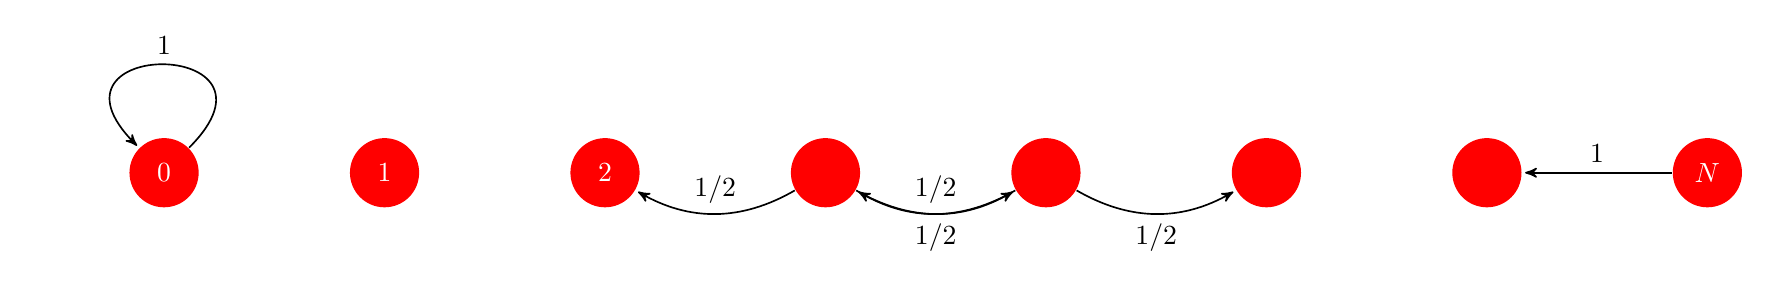
\begin{tikzpicture}[->,>=stealth',shorten >=1pt,auto,node distance=2.8cm,
                    semithick]
  \tikzstyle{every state}=[fill=red,draw=none,text=white]

  \node[state] (A)              {$0$};
  \node[state] (B) [right of=A] {$1$};
  \node[state] (C) [right of=B] {$2$};
  \node[state] (D) [right of=C] {};
  \node[state] (E) [right of=D] {};
  \node[state] (F) [right of=E] {};
  \node[state] (G) [right of=F] {};
  \node[state] (H) [right of=G] {$N$};

  \path (A) edge [loop, above]            node {1} (A)
        (D) edge [bend left, above] node {1/2} (C)
            edge [bend right, above] node {1/2} (E)
        (E) edge [bend left, below] node {1/2} (D)
            edge [bend right, below] node {1/2} (F)
        (H) edge [above]             node {1} (G);
\end{tikzpicture}

\end{document}
